\documentclass{article}

\usepackage{amsmath}
\usepackage{amssymb}
\usepackage{graphicx}
\usepackage{multicol}
\setlength{\parskip}{1em}

\begin{document}

	\title{ENUME project report\\Project C: least-squares approximation \\
	and solving systems of differential equations}
	\author{Michał Szopiński\\\\
	https://github.com/Lachcim/szopinski-enume\\
	Project number 60}
	\date{January 7, 2021}
	\maketitle
	
	\numberwithin{equation}{section}
	
	\setcounter{section}{-1}
	\section{Abstract}
	
	This project explores the numerical methods of function approximation
	and dynamic system analysis. The following concepts are discussed within
	this document:
	
	\begin{itemize}
		\item Performing the approximation of a function given by a set of
		discrete data points by a polynomial function of a given degree
		using the least-squares approach
		\item Determining the trajectory of an object whose motion is
		defined by a set of ordinary differential equations using the RK4
		and Adams PC algorithms
	\end{itemize}
	
	\newpage
	
	\section{Task 1: Least-squares approximation}
	
	\subsection{Overview}
	
	The goal of this task was to find the approximation of a function given
	by a set of data points. The approximating function was to be a
	polynomial of varying degree (several degrees were to be tested). The
	least-squares problem was to be solved using QR factorization.
	
	\subsection{Implementation}
	
	\subsubsection{Finding the vector $\widehat{a}$}
	
	The approximating function is given by:
	\begin{equation}
		a_0 + a_1x + a_2x^2 + a_3x^3 + \ldots + a_nx^n = 0
	\end{equation}
	where $n$ is the degree of the approximating polynomial. The goal of the
	approximation is to find a vector $\widehat{a} = [ a_0; a_1; \ldots;
	a_n ]$ such that:
	\begin{equation}
		(\forall{a \in \mathbb{R}^n})\quad
		\left\Vert y - A\widehat{a} \right\Vert_2 \leq
		\left\Vert y - Aa \right\Vert_2
	\end{equation}
	where $A\widehat{a}$ forms the vector of values of the approximating
	function at each data point, and $y$ is the vector of the values of the
	data points. In other words, the goal is to minimize the Euclidean norm
	of the difference between the approximating function and the data
	points.
	
	The most optimal vector $\widehat{a}$ can be obtained by calculating the
	derivative of the error function with respect to $a_n$ and equating it
	to zero. The resulting system of equations, called the
	\textit{normal equations}, has a unique solution: the vector
	$\widehat{a}$.
	
	\subsubsection{Solving normal equations using QR decomposition}
	
	Although this system could be solved directly using Gaussian elimination
	or an iterative method, the matrix describing this system, called Gram's
	matrix, tends to have a high condition number, which limits the accuracy
	of the solution. For this reason, the matrix $A$ is defined:
	\begin{equation}
		A = \begin{bmatrix}
			1 & x_0 & (x_0)^2 & (x_0)^3 & \dots & (x_0)^n \\
			1 & x_1 & (x_1)^2 & (x_1)^3 & \dots & (x_1)^n \\
			1 & x_2 & (x_2)^2 & (x_2)^3 & \dots & (x_2)^n \\
			\vdots & \vdots & \vdots & \vdots & \ddots & \vdots \\
			1 & x_N & (x_N)^2 & (x_N)^3 & \dots & (x_N)^n
		\end{bmatrix}
	\end{equation}
	where $x_N$ is the x-axis position of the $N$-th data point. The system
	of natural equations can then be expressed in terms of $A$ as follows:
	\begin{equation}
		(A^TA)\widehat{a} = A^Ty
	\end{equation}
	The condition number of $A$ is equal to the square root of the condition
	number of the original Gram's matrix, which yields better numerical
	properties. Furthermore, this form lends itself nicely to being solved
	using QR factorization of $A$:
	\begin{equation}
		(R^TQ^T)(QR)\widehat{a} = (R^TQ^T)y
	\end{equation}
	By observing that $Q^TQ = I$ and $\det{R} \neq 0$, this equation can be
	further reduced to:
	\begin{equation}
		R\widehat{a} = Q^Ty
	\end{equation}
	As an optimization, the QR decomposition can be replaced with a $\bar{Q}
	\bar{R}$ decomposition, which is faster to calculate:
	\begin{equation}
		\bar{R}\widehat{a} = (\bar{Q}^T\bar{Q})^{-1}(\bar{Q}^T)y
		\label{eq:rq}
	\end{equation}
	Because $\bar{R}$ is an upper triangular matrix, the
	equation~\ref{eq:rq} can be easily solved using back-substitution.
	
	\subsubsection{Performing the $\bar{Q}\bar{R}$ decomposition of a
	matrix}
	
	The $\bar{Q}\bar{R}$ decomposition is done using the modified
	Gram-Schmidt algorithm. The decomposing function returns
	$(\bar{Q}^T\bar{Q})^{-1}$ as part of its output and the final
	normalization subroutine used for ordinary QR decomposition is skipped.
	
	\subsection{Program output}
	
	\subsubsection{Approximating function plots}
	
	\includegraphics[width=\textwidth]{approx0}
	\includegraphics[width=\textwidth]{approx1}
	\includegraphics[width=\textwidth]{approx2}
	\includegraphics[width=\textwidth]{approx3}
	
	\subsubsection{Approximation errors and Gram's matrix condition number}
	
	\begin{center}
		\begin{tabular}{|c|r|r|} 
			\hline
			Degree & Error & Condition number \\
			\hline
			0 & 26.9222 & 1 \\
			1 & 24.5645 & 10 \\
			2 & 5.3885 & 408.7796 \\
			3 & 0.8872 & 8558.4366 \\
			\hline
		\end{tabular}
	\end{center}
	
	\subsection{Observations}
	
	Increasing the degree of the approximating polynomial made it possible
	to obtain a better approximation, i.e. one with a lower Euclidean norm
	error. By degree 3, the polynomial approximated the data points nearly
	perfectly and further approximation yielded no significant improvements.
	
	Higher polynomial degrees also caused the condition number of the Gram's
	matrix to rise exponentially. This problem was mitigated by implementing
	the QR decomposition of the matrix A, which made it possible to
	calculate the solution to the set on normal equations with a better
	accuracy.
	
	\newpage
	\section{Task 2a: Trajectory calculation using fixed-step algorithms}
	
	\subsection{Overview}
	
	In this task, the goal was to compute the trajectory of an object whose
	motion is described by a system of differential equations:
	\begin{gather*}
		\begin{cases}
			\frac{dx_1}{dt} = x_2 + x_1(\frac{1}{2} - x_1^2 - x_2^2)\\
			\frac{dx_2}{dt} = -x_1 + x_2(\frac{1}{2} - x_1^2 - x_2^2)
		\end{cases}\\
		t \in [0; 15]\\
		x_1(0) = 0\\
		x_2(0) = 12
	\end{gather*}
	The system was to be solved using two fixed-step algorithms, RK4 and
	Adams PC ($P_5EC_5E$). Two step sizes were to be chosen -- an ``optimal"
	one and a larger, visibly differing one.
	
	\subsection{Implementation}
	
	Numerical methods of solving systems of differential equations involve
	computing the value of the solution for a set of arguments belonging to
	the prescribed interval. Based on a vector of initial values and a set
	of functions describing the derivative of the solution, the output is
	computed by integrating the derivative over a small interval, in this
	context called a step.
	
	These algorithms can be divided into single-step and multi-step methods.
	Single-step methods only consider one preceding data point of the
	solution to calculate the next point, whereas multi-step algorithms
	consider multiple predecessors.
	
	\subsubsection{4\textsuperscript{th}-order Runge-Kutta method (RK4)}
	
	A single iteration of any single-step method can be described by the
	following formula:
	\begin{equation}
		y_{n + 1} = y_n + h\Phi_f(x_n; y_n; h)
	\end{equation}
	Where $y$ is the output solution vector, $x$ is the argument vector and
	$h$ is the step size. The function $\Phi_f$ is specific to the applied
	algorithm and it uses the provided data to calculate the next output
	data point.
	
	The RK4 algorithm is defined as follows:
	\begin{align}
		\begin{split}
			\Phi_f(x_n; y_n; h) &= \frac{1}{6}(k_1 + k_2 + k_3 + k_4)\\
			k_1 &= f(x_n, y_n)\\
			k_2 &= f(x_n + \frac{h}{2}, y_n + \frac{h}{2}k_1)\\
			k_3 &= f(x_n + \frac{h}{2}, y_n + \frac{h}{2}k_2)\\
			k_4 &= f(x_n + h, y_n + hk_3)
		\end{split}
	\end{align}
	This algorithm is fairly simple to implement and produces visually
	acceptable results. Because neither the system nor the algorithm utilize
	the argument vector $x$, this parameter tends to be omitted in the
	implementation.
	
	\subsubsection{Adams PC method ($P_5EC_5E$)}
	
	Adams predictor-corrector is a much more complicated, multi-step method
	which uses which uses the following algorithm:
	\begin{enumerate}
		\item Predict:
			\begin{equation*}
				y^{[0]}_n = y_{n - 1} + h\sum_{j=1}^{5}\beta_j f_{n-j}
			\end{equation*}
		\item Evaluate:
			\begin{equation*}
				f^{[0]}_n = f(x_n, y^{[0]}_n)
			\end{equation*}
		\item Correct:
			\begin{equation*}
				y_n = y_{n - 1} + h\sum_{j=1}^{5}\beta^*_j f_{n-j}
				+ h\beta^*_0f^{[0]}_n
			\end{equation*}
		\item Evaluate:
			\begin{equation*}
				f_n = f(x_n, y_n)
			\end{equation*}
	\end{enumerate}
	This algorithm serves to efficiently implement the implicit Adams
	method. The predictor helps to do so by choosing a suitable starting
	point.
	
	\subsection{Program output}
	
	\subsubsection{RK4 solution plots}
	\includegraphics[width=\textwidth]{rk4x1}
	\includegraphics[width=\textwidth]{rk4x2}
	\includegraphics[width=\textwidth]{rk4traj}
	
	\subsubsection{Adams PC solution plots}
	\includegraphics[width=\textwidth]{adamspcx1}
	\includegraphics[width=\textwidth]{adamspcx2}
	\includegraphics[width=\textwidth]{adamspctraj}
	
	\newpage
	\subsection{Observations}
	
	For the Runge-Kutta method, the ``optimal" step size was 0.01, whereas
	the largest feasible step size obtainable was 0.013408. Above this
	limit, the integration diverged to the point where the trajectory
	coordinates quickly reached infinity. Adams PC exhibited similar
	behavior for step sizes above 0.01305.
	
	Analysis of the $x_2$ function reveals that it is extremely steep in the
	neighborhood of the initial conditions, reaching a derivative of -1722
	in the first iteration:
	\includegraphics[width=\textwidth]{x_2gradient}
	For this reason, the resulting trajectory graph is much denser (in terms
	of data points) near the final spiral than it is in the initial entry
	path.
	
	In comparison, the $x_1$ component is relatively flat in the
	neighborhood of the trajectory, with an initial derivative of 12:\\
	\includegraphics[width=\textwidth]{x_1gradient}
	
	This behavior likely serves to illustrate the necessity of the Lipschitz
	condition for the integrability of a function. An infinitely steep
	function cannot be integrated over a finite step, with additional
	limitations superimposed by the machine precision of the computing
	system.
	
	\newpage
	\section{Task 2b: Trajectory calculation using variable-step RK4}
	
	\subsection{Overview}
	
	This variant of the previous task aims to reimplement the RK4 algorithm
	with a variable step size determined by the double-step error
	estimation. The step size and the error estimation were to be plotted
	against time. Finally, the results were to be compared against a
	solution obtained with ODE45.
	
	\subsection{Implementation}
	
	There exists an inherent conflict of interest between decreasing the
	step size and increasing it -- smaller steps give more accurate results,
	but they increase computation time and accumulate floating-point errors.
	To solve this problem, the RK4 algorithm can be altered to dynamically
	change the step size so as to achieve a predetermined desired accuracy,
	in this case, a relative error of $10^{-10}$.
	
	To do so, the algorithm estimates the current approximation error on
	each step and calculates the step scaling factor $\alpha$. The error is
	estimated using the double-step method, where each iteration is computed
	with a single full-sized step and two half-sized steps. Its value is
	given by:
	\begin{equation}
		\delta_n(h) = \frac{y^{(2)}_n - y^{(1)}_n}{2^p - 1}
	\end{equation}
	where $y^{(q)}$ denotes the solution obtained after $q$ subsequent
	$\frac{1}{q}$-steps. The error of a single step multiplied by $\alpha$
	is equal to:
	\begin{equation}
		\delta_n(\alpha h) = \alpha^{p + 1} \cdot \delta_n(h)
	\end{equation}
	If $\delta_n(\alpha h)$ is substituted for the desired error
	$\varepsilon$, the above two equations can be combined to obtain:
	\begin{equation}
		\alpha = \left(\frac{\varepsilon}{\delta_n(h)}\right)
		^\frac{1}{p + 1}
	\end{equation}
	Finally, because $\varepsilon$ and $\delta_n$ are absolute errors, the
	desired error can be formulated in terms of a relative and an absolute
	input parameter:
		\begin{equation}
		\alpha = \left(\frac
		{|y^{(2)}_n| \cdot \varepsilon_{rel} + \varepsilon_{abs}}
		{|\delta_n(h)|}\right)
		^\frac{1}{p + 1}
	\end{equation}
	Lastly, the obtained scaling factor $\alpha$ is multiplied by a safety
	factor of 0.9 to account for errors in the error estimation itself.
	
	A flowchart of the variable-stepped RK4 algorithm:\\
	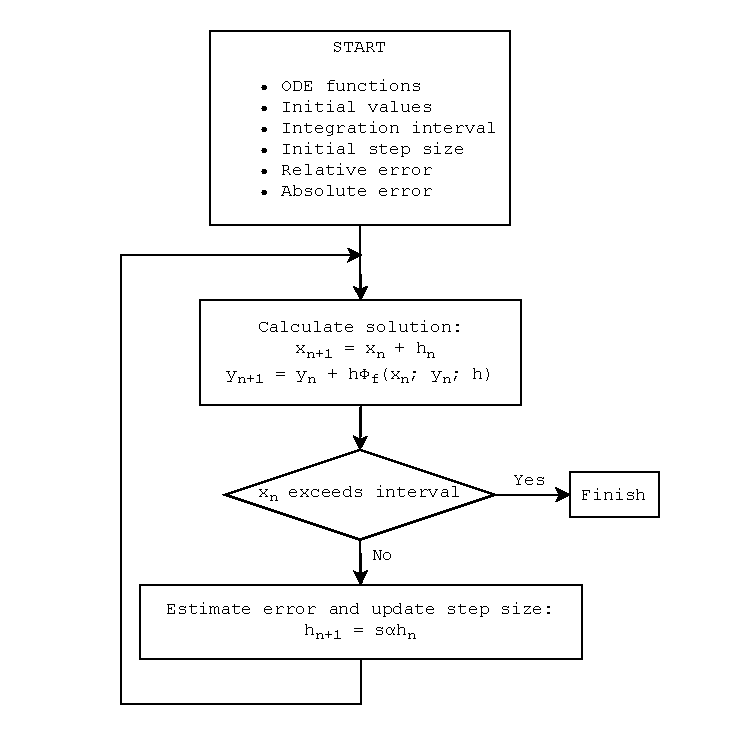
\includegraphics[width=\textwidth]{flowchart}
	
	\subsection{Program output}
	
	\includegraphics[width=\textwidth]{rk4autotraj}
	\includegraphics[width=\textwidth]{rk4sizes}
	\includegraphics[width=\textwidth]{rk4errors}
	\includegraphics[width=\textwidth]{ode45}
	
	\newpage
	\subsection{Observations}
	
	The variable-step Runge-Kutta method provided an optimal solution
	visually identical to that returned by Matlab's ODE45. As seen on the
	step size plot, the step size was automatically increased for regions
	with greater derivatives and decreased where the functions changed
	slowly.
	
	The approximation error plot reveals that the algorithm succeeded in
	maintaining an absolute error of $10^{-10}$. The only anomaly visible
	at the start of the plot resulted from a poorly chosen initial step
	size.
	
	Although the typical specification of a variable-step RK4 algorithm
	calls for the implementation of a minimal step size $h_{min}$, this was
	unnecessary for the purpose of this experiment -- the function was
	successfully graphed with the desired accuracy. A more generic
	implementation could benefit from an $h_{min}$ that would prevent
	prohibitive computation times.
	
\end{document}
